\subsection{Effects of supervision targets and checkpoint selection}
The primary comparison concerns whether the supported-category vote distribution improves selective predictions beyond preserving the dominant target probability. At 80\% coverage, validation-selected Swin-T models trained with Soft have mean complete-vote disagreement of 23.68\%, compared with 24.06\% for Uniform (Table~\ref{tab:primary}). The paired Soft-minus-Uniform difference is -0.38 pp, with a conditional 95\% interval of [-0.64, -0.07]. This is a modest advantage over the matched softening control; each model selects its own accepted images.
\begin{table}[t]
\caption{Selected-checkpoint risk at 80\% coverage (2,620 of 3,275 images). Risk is mean $\pm$ sample SD; components are mean percentage points}\label{tab:primary}
\centering\begin{tabular}{lrrrr}\toprule
Targets & Risk (\%) & Unsupported & Ambiguity & Excess\\\midrule
Hard & $26.30 \pm 1.04$ & 6.65 & 16.14 & 3.51\\
Tie-hard & $25.82 \pm 0.58$ & 6.67 & 16.03 & 3.13\\
Uniform & $24.06 \pm 0.10$ & 6.41 & 15.41 & 2.24\\
Tie-Uniform & $24.27 \pm 0.17$ & 6.47 & 15.46 & 2.35\\
Soft & $23.68 \pm 0.07$ & 6.55 & 15.01 & 2.13\\
\bottomrule\end{tabular}\par
Accepted identities differ; components provide accounting, not causal attribution.
\end{table}


The retained comparisons with hard targets show why the control matters. Soft minus Hard is -2.61 pp (conditional 95\% interval [-2.98, -2.19]), substantially larger than the primary Soft-minus-Uniform contrast. Tie-hard minus Hard is -0.47 pp (interval [-0.80, -0.12]), while Soft minus Tie-hard is -2.14 pp (interval [-2.49, -1.76]). These secondary intervals describe sensitivity to the target construction, rather than additional primary hypothesis tests.

The direction of the primary Swin-T contrast persists when the checkpoint is retained after 12 epochs instead of selected by validation distance. Soft minus Uniform is then -0.32 pp (conditional 95\% interval [-0.63, -0.05]); Soft minus Hard is -1.35 pp (interval [-1.72, -1.05]). Table~\ref{tab:sensitivity} reports the absolute risks at both checkpoint states. This comparison changes checkpoint selection, not the training budget or objective.
\begin{table}[t]
\caption{Selected versus fixed epoch-12 complete-vote risk at 80\% coverage (\%); means across three paired seeds}\label{tab:sensitivity}
\centering\begin{tabular}{lrr}\toprule
Targets & Selected & Epoch 12\\\midrule
Hard & 26.295 & 24.983\\
Tie-hard & 25.824 & 24.576\\
Uniform & 24.062 & 23.949\\
Tie-Uniform & 24.272 & 23.939\\
Soft & 23.684 & 23.632\\
\bottomrule\end{tabular}\par

\end{table}


The tie-preserving control gives the same qualitative result for Swin-T. Soft has lower disagreement than Tie-Uniform at both checkpoint states, with conditional intervals below zero (Table~\ref{tab:backbones}). Unlike Uniform, Tie-Uniform does not favor a single category when the highest vote counts are tied. Both controls nevertheless differ from Soft in entropy and aggregate class proportions, so these comparisons do not isolate the effect of minority-category identity alone. The supplementary learning and selection curves retain all training trajectories; loss magnitudes across different target constructions are not directly comparable measures of fitting quality.

Figure~\ref{fig:difference} places the primary endpoint in the broader coverage range. It is a descriptive comparison using each model's own confidence ranking, not an additional confirmatory test.
\begin{figure}[tp]\centering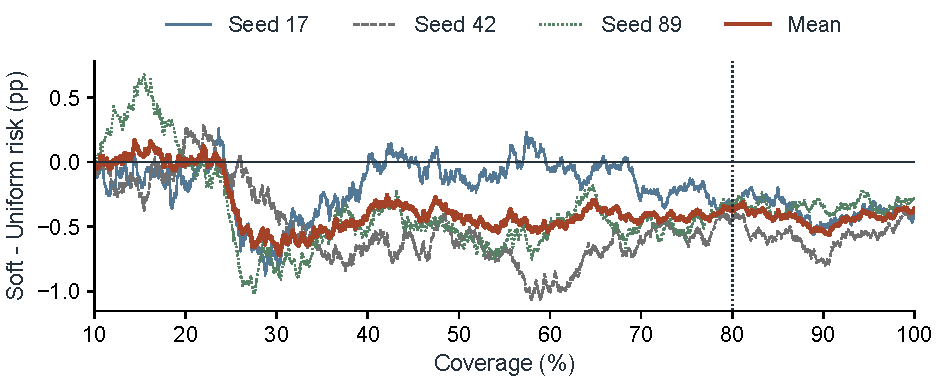
\includegraphics[width=\linewidth]{submission_reader_2026_10_13/source/figures/Fig5.pdf}
\caption{Soft-minus-Uniform complete-vote disagreement versus common coverage. Thin curves show paired seeds; the thick curve shows their mean. Each model uses its own ranking, rather than an identical accepted-image set. The vertical marker identifies the primary 80\% endpoint. No simultaneous uncertainty band is estimated}\label{fig:difference}\end{figure}
